% !TeX program = xelatex

\documentclass{beamer}

\usepackage[utf8]{inputenc}
\usepackage{graphicx}
\usepackage{listings}

%Tamarin Code Highlighter
\definecolor{dartmouthgreen}{rgb}{0.05, 0.5, 0.06}
\lstdefinelanguage{Tamarin}{
	alsoletter={-},
	keywords=[1]{},
	otherkeywords={[, ], --, ->, [, \t\,},
	keywords=[2]{let, in, exists-trace},
	keywords=[3]{rule, lemma, Ex, All, not},
	keywords=[4]{RevDHQ},
	keywordstyle=[1]{\color{black}\bfseries},
	keywordstyle=[2]{\color{dartmouthgreen}\bfseries},
	keywordstyle=[3]{\color{blue}\bfseries},
	keywordstyle=[4]{\color{magenta}\itshape\bfseries},
	string=[b]{'},
	stringstyle=\color{red},
	numbers=left,
	numberstyle=\scriptsize,
	stepnumber=1,
	numbersep=8pt,
	comment=[l]{//},
	morecomment=[s]{/*}{*/},
	commentstyle=\color{gray!75},
	basicstyle=\normalfont\ttfamily,
	breakatwhitespace=false,         % sets if automatic breaks should only happen at whitespace
	breaklines=true,                 % sets automatic line breaking
	captionpos=b                    % sets the caption-position to bottom
}

% for table
\usepackage{bbding}
\usepackage{threeparttable,tabularx}
\usepackage{booktabs}
\newcommand{\yes}{\textcolor{dartmouthgreen}{\raisebox{-2pt}{\CheckmarkBold}}}
\newcommand{\no}{\textcolor{red}{\raisebox{-2pt}{\XSolidBrush}}}

\lstset{
  frame=single,
  basicstyle=\footnotesize\ttfamily,
  captionpos=b,
  tabsize=2,
}
\beamertemplatenavigationsymbolsempty
\setbeamertemplate{footline}{%
\insertframenumber{}/\inserttotalframenumber}


%Information to be included in the title page:
\title{A formal analysis of IKEv2's post-quantum extension}
\usecolortheme{dove}
\author{Stefan-Lukas Gazdag, Sophia Grundner-Culemann,\\
    Tobias Guggemos, \underline{Tobias Heider},\\
    Daniel Loebenberger}
\institute{ACSAC2021}
\date{12/08/21}

\setbeamertemplate{itemize items}[circle]
\setbeamertemplate{itemize subitem}[default] \begin{document}

\begin{frame}[noframenumbering, plain]
	\titlepage
\end{frame}

\begin{frame}
\frametitle{The IKEv2 Protocol}
\centering
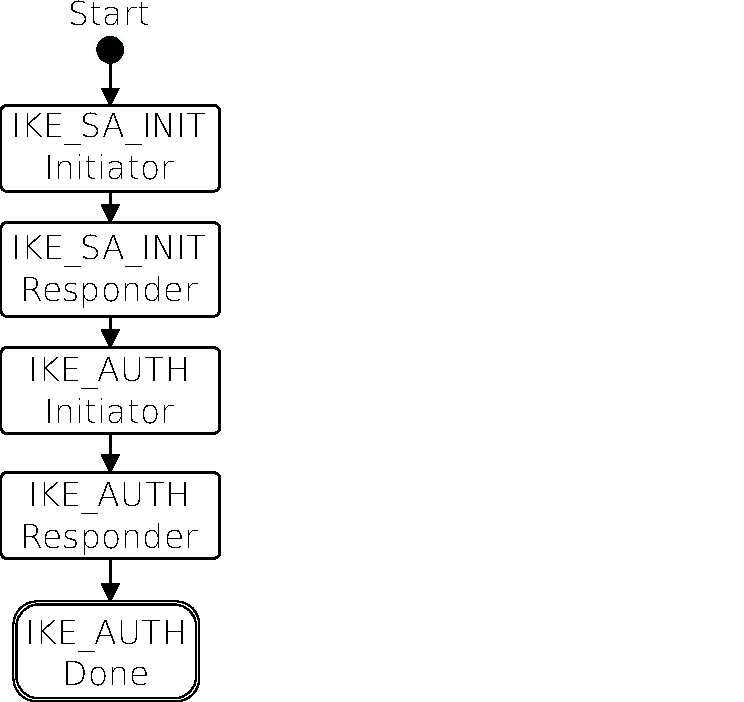
\includegraphics[width=.8\textwidth]{statemachine-classic.pdf}
\end{frame}

\begin{frame}
\frametitle{Post-Quantum IKEv2}
\centering
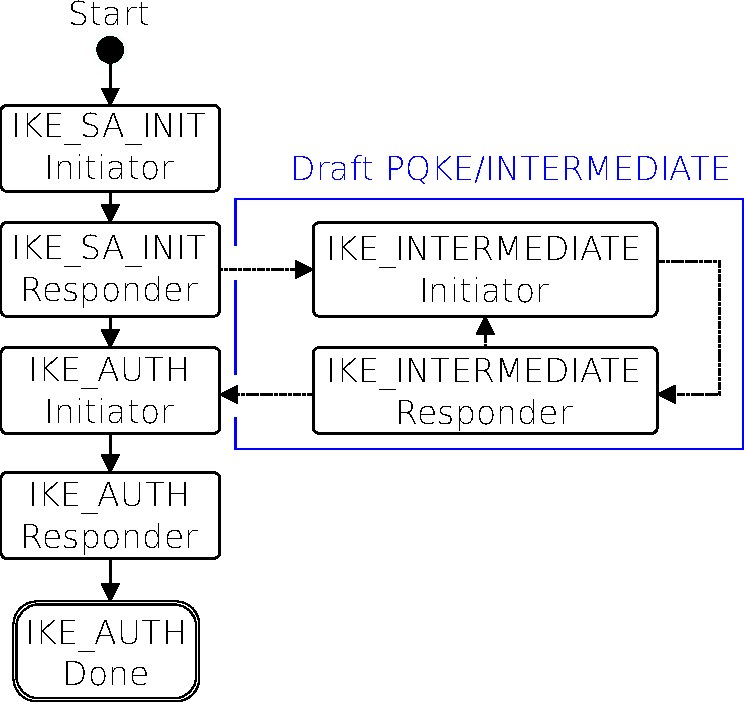
\includegraphics[width=.8\textwidth]{statemachine-pq.pdf}
\end{frame}

\begin{frame}
\frametitle{The Tamarin Prover}
\underline{\text{Idea:}}
\begin{itemize}
	\item symbolic modeling and protocol analysis
	\pause
	\item transition system
	\begin{itemize}
		\item ``exists-trace''
		\item ``all traces fulfill ... ''
	\end{itemize}
	\pause
	\item support of crypto primitives and concepts:
	\begin{itemize}
		\item hashing
		\item symmetric and asymmetric encryption
		\item signing
		\item Diffie-Hellman
	\end{itemize}
	\pause
	\item real-world impact, e.g.:
	\begin{itemize}
		\item during TLS 1.3 standardization
		\item Wireguard
	\end{itemize}
\end{itemize}
\end{frame}

\begin{frame}[fragile]
\frametitle{The Tamarin Language}

\begin{lstlisting}[language=Tamarin]
rule Register_pk:
  [ Fr(~ltk) ]
  --[HaveLtk($A)]->
  [ !Ltk($A, ~ltk), !Pk($A, pk(~ltk)) ]

lemma exists_pk: exists-trace
  " Ex $A #i.
    HaveLtk($A) @ #i
  "
\end{lstlisting}
% \begin{lstlisting}[language=Tamarin]
% rule reveal_dh:
% [ !DHtoReveal($I, k) ]
% --[RevDH($I)]->
% [ Out(k) ]
% \end{lstlisting}

\end{frame}

\begin{frame}[fragile]
\frametitle{Modeling IKEv2}
\begin{lstlisting}[language=Tamarin]
rule IKE_SA_INIT_I:
  ...
rule IKE_SA_INIT_R:
  ...
rule IKE_AUTH_I:
  ...
rule IKE_AUTH_R:
  ...

lemma exists_session : exists-trace
  "Ex I R spi # i #j keymat .
  Completed(spi, I, 'initiator', R, keymat) @ #j &
  Completed(spi, R, 'responder', I, keymat) @ #i &
  #i < #j"
\end{lstlisting}
\end{frame}

\begin{frame}
\frametitle{IKEv2 Security Model}

\underline{\text{Security properties:}}
\begin{itemize}	
	\item Consistency
	\item Key secrecy
	\item Identity Protection
	\item Agreement \smallskip
	\begin{itemize}
		\item Aliveness \textit{(of Initiator and of Responder)}
		\item Weak Agreement \textit{(of Initiator and of Responder)}
		\item Agreement \textit{(of Initiator and of Responder)}		
	\end{itemize}
\bigskip
$\dots$ against a Dolev-Yao attacker
	
\end{itemize}
\end{frame}

\begin{frame}[fragile]
	\frametitle{Modeling PQ-IKEv2}
\begin{lstlisting}[language=Tamarin]
rule IKE_INTERMEDIATE_I:
  ...

rule IKE_INTERMEDIATE_R:
  ...

rule reveal_dhq:
  [ !DHQtoReveal($I, k) ]
  --[RevDHQ($I)]->
  [ Out(k) ]
\end{lstlisting}
	
\end{frame}

\begin{frame}
\frametitle{Result}
\begin{table}[t]
\resizebox{\textwidth}{!}{
	\begin{tabular}{m{4cm}ccccc}
		\toprule
		& none & I eph. & R eph. & I static & R static \\
		\midrule
		Consistency & \yes & \yes & \yes & \yes & \no \\
		\hline
		Key secrecy & \yes & \no & \no & \yes & \no \\
		\hline
		\uchyph=0 Identity Protection & \yes & \no & \no & \no & \yes \\
		\hline
		Aliveness\_I & \yes & \yes & \yes & \yes & \no \\
		Aliveness\_R & \yes & \yes & \yes & \yes & \no \\
		\hline
		\uchyph=0 Weak Agreement\_I & \yes & \no & \no & \yes & \no \\
		\uchyph=0 Weak Agreement\_R & \no & \no & \no & \no & \no \\
		\hline
		Agreement\_I & \yes & \no & \no & \yes & \no  \\
		Agreement\_R & \no & \no & \no & \no & \no \\
		\bottomrule
	\end{tabular}
}
\caption[]{\textbf{Implications of key compromise:} Each entry indicates whether the security property of the corresponding row is achieved (\yes{}) or not (\no{}) if the key of the corresponding column is compromised. }
\end{table}
\end{frame}

\end{document}
